\documentclass{bioinfo}
\copyrightyear{2017}
\pubyear{2017}




%%% Additional Macro and command.
\usepackage{url}
\newcommand{\pkg}[1]{{\fontseries{b}\selectfont #1}}
\makeatletter
\newcommand\code{\bgroup\@makeother\_\@makeother\~\@makeother\$\@codex}
\def\@codex#1{{\normalfont\ttfamily\hyphenchar\font=-1 #1}\egroup}
\makeatother
\let\proglang=\textsf
%%% End of additional Macro and command.


\newcommand{\package}{\textbf{AnaCoDa }} % need that whitespace there for text flow
\usepackage{natbib}

%%% Start here.
\begin{document}


\firstpage{1}

\title[AnaCoDa]{AnaCoDa: Analyzing Codon Data with Bayesian mixture models}
\author[
Landerer \textit{et~al}]{Cedric Landerer\,$^{1,2}$\footnote{
to whom correspondence should be addressed
},
Alexander Cope\,$^{3,5}$
Russell Zaretzki\,$^{2,4}$, and
Michael Gilchrist\,$^{1,2}$
}
\address{$^{1}$
Department of Ecology and Evolutionary Biology,
$^{2}$National Institute for Mathematical and Biological Synthesis,
$^{3}$Genome Science and Technology
$^{4}$Department of Statistics, Operations, and Management Science,
University of Tennessee, Knoxville, TN, USA,
$^{5}$Oak Ridge National Laboratory, Oak Ridge, TN, USA} 
\history{Received on XXXXX; revised on XXXXX; accepted on XXXXX}

\editor{Associate Editor: XXXXXXX}

\maketitle

\begin{abstract}

%\section{Summary:}
%\pkg{\package} is a fast and reliable collection of codon models, which currently estimate terms related to mutation, selection, and other population genetics parameters of interest from codon counts.

% I made this edit because not all models are evolutionary models

\pkg{\package} is a fast and reliable software for estimating biological parameters from codon count data, such as selection against translation inefficiency, nonsense error rates, and ribosome pausing times.
\package provides an adaptive Bayesian MCMC algorithm, fully implemented in C++ to improve computational performance with an ergonomic R interface to improve usability. 
\package also follows a generic object-oriented design to allow users to extend the framework and implement their own models for analyzing biological data.
%Old------------------------------------------------------
%Currently implemented models can be used to analyze coding sequence data and ribosome foot printing counts to estimate parameters related to ribosome overhead costs, nonsense error rates, and ribosome pausing times. 
%In addition, \package features mixture distributions for parameters, allowing users to set or estimate mixture assignment for groups sharing population level parameters, allows for simulation under the provided models and implements check-pointing functionality to restart runs if necessary. 
%Edit-----------------------------------------------------
Current models within \package can accurately estimate relevant parameters given either coding sequences or ribosome foot-printing data, depending on the model.
However, these models are capable of using other data, such as empirical measurements of gene expression, to better inform parameter estimates.
\package implements a mixture distribution for parameters shared across genes, allowing these parameters to be estimated under the assumption of different biological conditions and used to categorize genes into different sets.
In addition, \package includes the ability to simulate data, visualize results, and revisit previous runs should further analysis be needed. 

\section{Availability:}
\pkg{\package} is freely available under the Mozilla Public License 2.0
on CRAN (\url{http://cran.r-project.org/package=anacoda}).

\section{Contact:} \href{cedric.landerer@gmail.com}{cedric.landerer@gmail.com}
\end{abstract}


\section*{Introduction}
The exponential increase in publicly available genomes over the past decade and the addition of novel technologies produced a vast amount of data for researchers.  
This influx of raw data necessitates the development of computational tools for extracting biological information. 
Models have to be developed and provided to the public in easy to use software to allow researchers to analyze classical sequence data as well as novel data like ribosome foot-printing counts.

Here, we describe an open-source software implemented in R \citep{rcore} that allows researchers to analyze genome-scale data like coding sequences and ribosome foot-printing data in a Bayesian framework under various models. 
\package implements an adaptive Gibbs sampler within a Metropolis-Hastings Monte Carlo Markov Chain (MCMC) approach. This allows for the incorporation of prior knowledge and easy sampling from the posterior distribution to estimate parameter values and quantify the degree of uncertainty in these estimates.
Currently, \package provides three models to analyze codon counts obtained from coding sequences or ribosome foot-printing experiments. However, \package provides a modular infrastructure such that additional genome scale or even phylogenetic models can be integrated. 
\package provides a generic mixture distribution option to all implemented models, allowing for the automatic categorization of data based on differences in the posterior distributions of the relevant parameters.

The \package framework groups the provided data by gene and by codon, and differentiates three types of parameters: (1) shared parameters like codon parameters, (2) gene parameters like gene ordering, and (3) hyper-parameters. 
For all models, estimates of each type of parameter are conditioned on the other two types. 
This Gibbs sampling approach allows for a reduction in dimensionality, increasing sampling efficiency and computational performance.
Shared parameters are shared across all genes. These parameters are shared across all genes within a set of genes. Shared parameters are also used to automatically or manually assign genes into various sets. The number if sets has to be provided as well as an initial of fixed assignment.
Estimation of the set assignment provides the probability of a gene being assigned to a set allowing the user to asses the uncertainty in each assignment.
Gene-specific parameters are estimated independently for each gene. If the population specific parameters are used to classify genes into population, a gene specific parameter is estimated assuming the gene being assigned to each cluster. This allows to test hypothesis about gene specific parameters under various conditions, represented by different categories.
The inclusion of hyperparameters, like parametric prior distributions, allows for the implementation of hierarchical models.


\begin{figure*}[!tpb]
\centering
 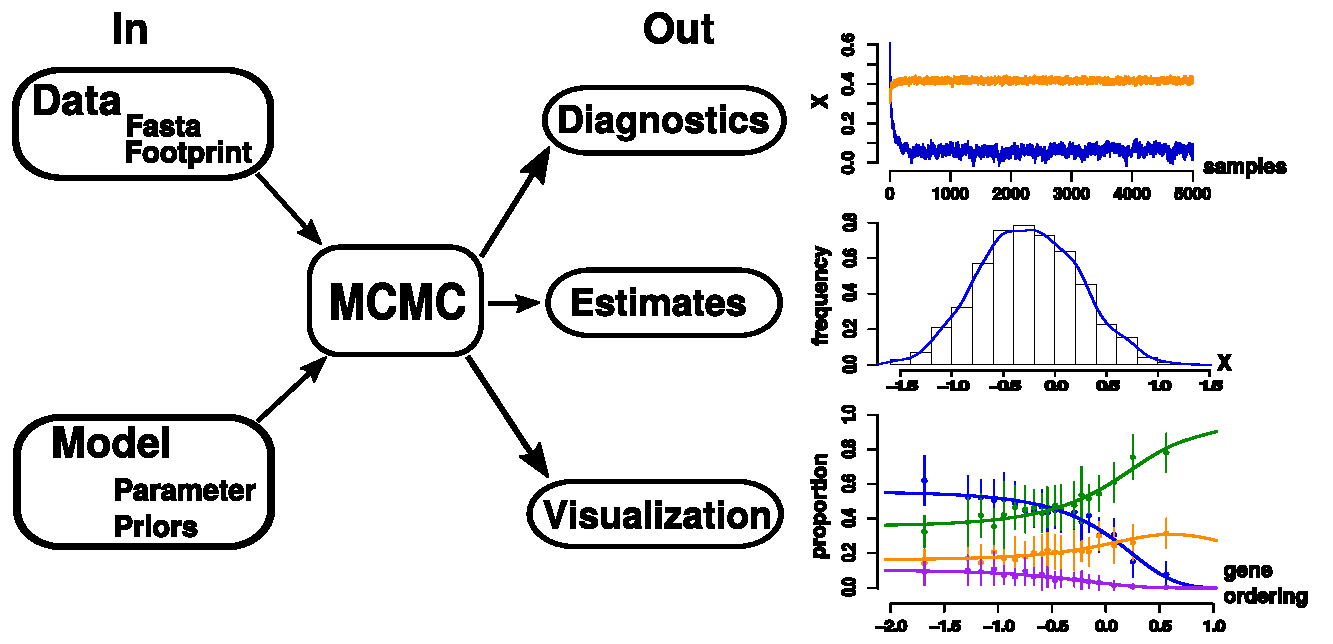
\includegraphics[width=5in]{workflow_croped.pdf}
\vspace{-0.2cm}
\caption{\textbf{Package overview and plotting functionality.} \package \textbf{Illustration of the angus workflow.} 
\package allows for the easy estimation of population genetics parameters from genome scale data such as CDS or ribosome footprints. 
Furthermore, \package provides functionality for MCMC diagnostics and visualization. 
}
\label{fig:plotbin}
\end{figure*}

\section*{Features}
\package provides an interface written in R, a freely available programming language noted for its ease of use for even inexperienced programmers. 
As a result, \package is accessible to researchers with minimal computational experience. 

The \package interface is designed for quick and efficient data analysis.
Generally, the only input needed for fitting a model to the data are protein-coding nucleotide sequences in the form of a FASTA file or a flat-file containing codon counts obtained from ribosome foot-printing experiments. 
If available, users may also provide empirically estimated values of gene expression as an additional guide for a model.
\package also provides visualization functionality, including plotting functions to compare parameter estimates for different mixture distributions and display codon usage patterns (Figure 1). In addition, diagnostic functions such as those for calculating and visualizing the degree of autocorrelation are provided.

Users are able to simulate data, such as protein-sequences, with \package. 
During model development, simulated data is useful for verifying the model. 
%If the model is working as expected, fitting the model to simulated data will result in parameter estimates approximately equal to the parameters used for the simulations. 
In addition, simulating data under different conditions allows the user to explore model behavior. 
Different conditions can include the addition or elimination of parameters, or simply allowing a set of parameter values to vary.
Simulated data obtained from various conditions can be compared to real data as a way to assess model adequacy.
Significant differences between the simulated and real data suggests the current set of parameters or the model as a whole do not accurately reflect the underlying biological mechanisms.

\package has built-in features designed to improve the performance of the implemented MCMC approach. 
For example, the implemented MCMC approach automatically adapts the proposal width for sampled parameters, improving sampling efficiency of the MCMC and computational performance.
In addition, \package is capable of thinning the MCMC chain, meaning only every $k^{th}$ sample is kept. 
Thinning increases the effective number of samples by reducing the auto-correlation between samples and reduces the amount of memory required by the underlying data structures. 

To protect users in the case of an abrupt ending to a run or failure of the MCMC to converge, \package outputs restart files throughout the course of the run. 
This allows the user to begin a MCMC based on the state of another MCMC at a previous time point. 
\package is able to create file representations of the Parameter and MCMC objects, which can be loaded into the R environment for further analysis and visualization of previous runs.

\subsubsection*{Mixture distributions}
Mixture distributions are commonly used when a data set is comprised of sub-populations or clusters which can be described by mixing various distribution \citep{gelman2013}. 
\package allows all implemented models with the ability to utilize mixture distributions for all population specific parameters like codon specific mutation and selection bias in the case of the ROC model. 
The separation of gene specific and population specific parameters creates the necessity to estimate a gene specific parameter for each possible cluster a gene can be assigned to. 
%As all implemented model contain gene specific parameters (e.g. protein production rate) in addition to population specific parameters (e.g. mutation) we extended the mixture approach implemented in \package to incorporate the need for a gene specific parameter. 
%Therefore, the protein production rate of each gene is estimated assuming it in each possible mixture distribution. 
This approach allows genes to be categorized based on differences in population specific parameters, like codon-specific mutation and selection biases, making \package ideal to ask questions about intra-genomic or even within-gene heterogeneity in mutation and selection patterns (see Landerer et al. XXXX for application). 

 
\subsubsection*{Available models}
\package currently provides codon models for analyzing genome scale data.
The ROC model implements the work presented by Gilchrist et al. (2015), which reliably estimates selection on \underline{r}ibosome \underline{o}verhead \underline{c}ost, mutation bias and allows for the inference of protein synthesis rates. The ROC model is an extension of work by Shah \& Gilchrist (2011) \citep{shah2011} and  Wallace et al (2013) \citep{wallace2013}. 
%The NSE model is focused on the estimation of \underline{n}on-\underline{s}ense \underline{e}rror rates and accounts for the position of a codon in the sequence. Codons found later in the sequence are assumed to be under stronger selection against non-sense errors, as total energy investment is increasing along the sequence.
This model allow for the separation of effects of mutation and selection based on gene ordering by protein synthesis rate, and the added mixture distribution allows for gene clustering based on these effects.
Furthermore, \package implements a Pausing (PA) model to extract information on ribosome pausing times from ribosome foot-printing data. The PA model assumes that ribosome foot-print counts are inverse proportional to pausing time allowing for the estimation of the distribution of ribosome pausing times for each codon. 

%\subsubsection*{Writing extensions}
%Users are welcome and encouraged to incorporate their own codon models into \package. The object-%oriented paradigm of C++ allowed for the implementation of a general framework for creating new models %to analyze genomic data. All implemented models in \package are encapsulated such that they share %certain commonalities. This allows for the creation of new models within the same framework. Generally, %these models can be added by creating appropriate subclasses of the Parameter and Model classes provided %by the current framework. These subclasses should include the additional functionality required for %these models. 

\package defines an interface to connect a model with the implemented MCMC algorithm. 
By following this general interface, researchers are easily able to add their own models to analyze sequence and foot-printing data or other data-types.
Researchers are able to create their own model, implementing the provided interface and inheriting functionality shared with other models.
Functionality unique to a model must be contained within the new model. 

\subsubsection*{Computational performance}
Although \package is provided as an R package, the main computational work is implemented in C++ and can be, if desired, compiled as a standalone software.
R does not provide native C++ support, but the R package Rcpp allows for the exposure of whole C++ classes as modules to R \citep{rcpp_package}.
This eliminates time consuming data transfer between the R environment and the C++ core during runs, resulting in improved computational performance and allowed for a fully object-oriented code design \cite{ood_book}. 
As expected, the runtime of \package scales linear with genome size and number of iterations, and polynomial with the number of mixture distributions in the data set. The polynomial increase in the number of mixture distributions is explained by the necessity to estimate the protein production rate for each gene in each mixture distribution, as it is a gene specific parameter and the probability of a gene being assigned to a mixture has to be conditioned on it.

\bibliographystyle{natbib}
\bibliography{bioinfo}
\end{document}
